\normaltrue \difficilefalse \tdifficilefalse
\correctiontrue

%\UPSTIidClasse{11} % 11 sup, 12 spé
%\newcommand{\UPSTIidClasse}{11}

\exer{Diagramme de Bode$\star$ \label{C2:02:510}}
\setcounter{numques}{0}
\UPSTIcompetence[2]{C2-02}
\index{Compétence C2-02}
\index{Diagramme de Bode}
\ifcorrection
\else
\textbf{Pas de corrigé pour cet exercice.}
\fi


\ifprof 
\else
 \fi
 
\question{Tracer le diagramme de Bode de la fonction de transfert suivante : $F_1(p)=\dfrac{15}{1+10p}$.}

\ifprof

\textbf{Tracer asymptotique}

\begin{center}
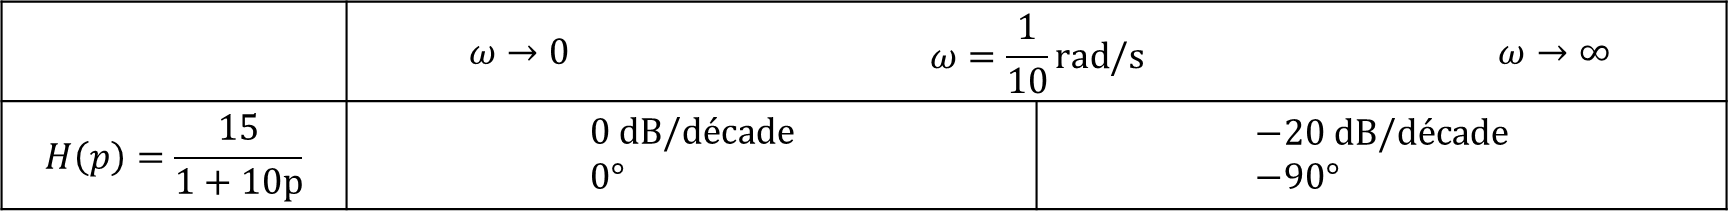
\includegraphics[width=.9\linewidth]{tab_01}
\end{center}


\textbf{Positionnement du diagramme de gain}
Lorsque que $\omega$ tend vers 0, le gain tend vers $20 \log 15 = \SI{23,5}{dB}$.

\begin{center}
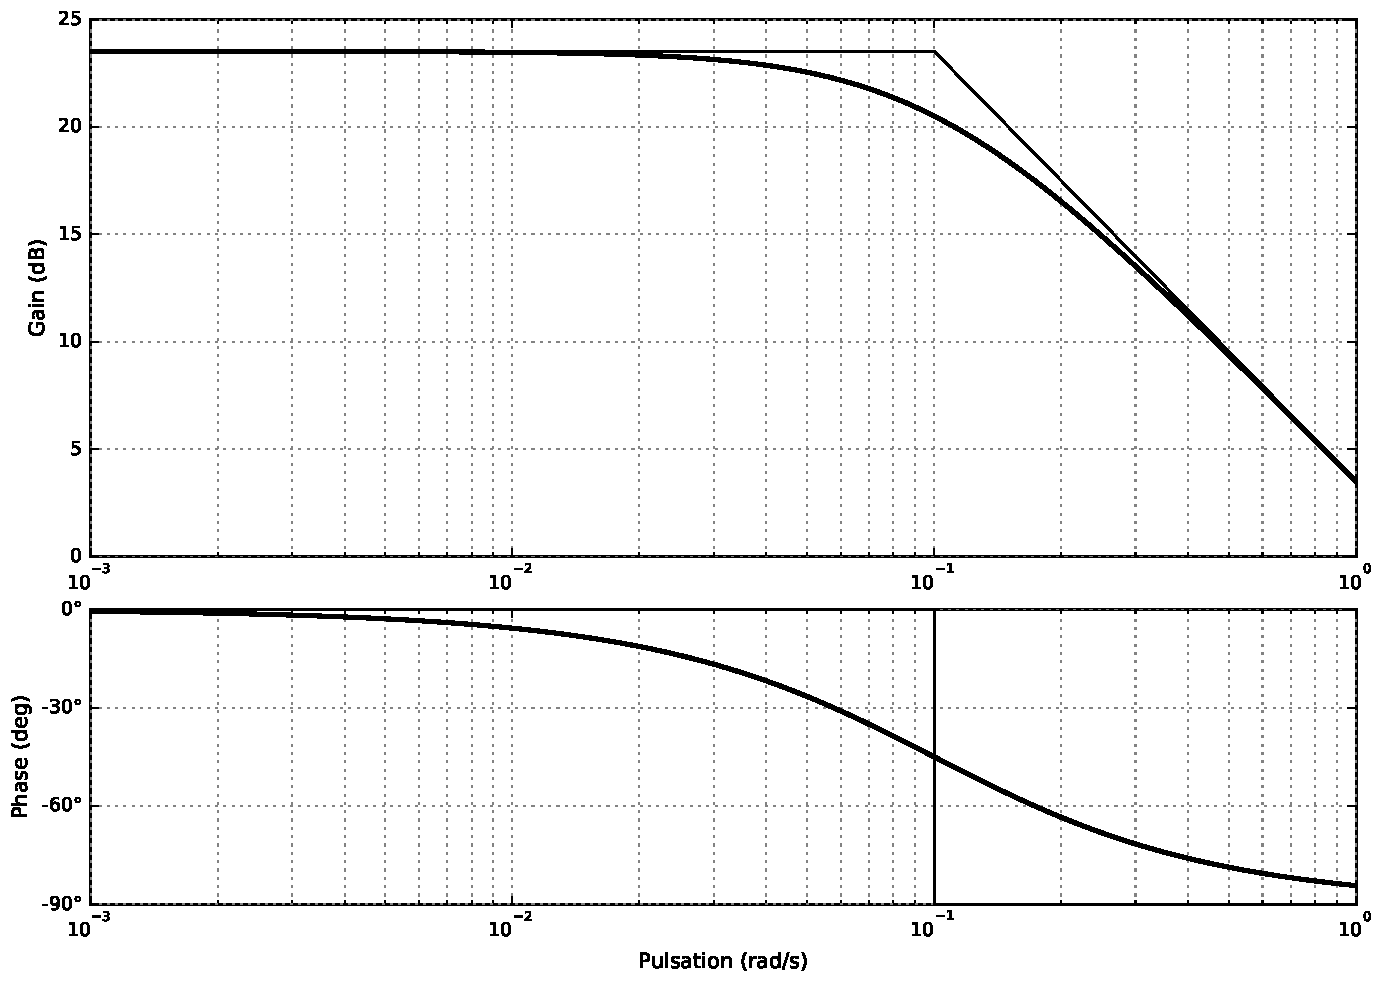
\includegraphics[width=.9\linewidth]{bode_01}
\end{center}

\else 
\begin{center}
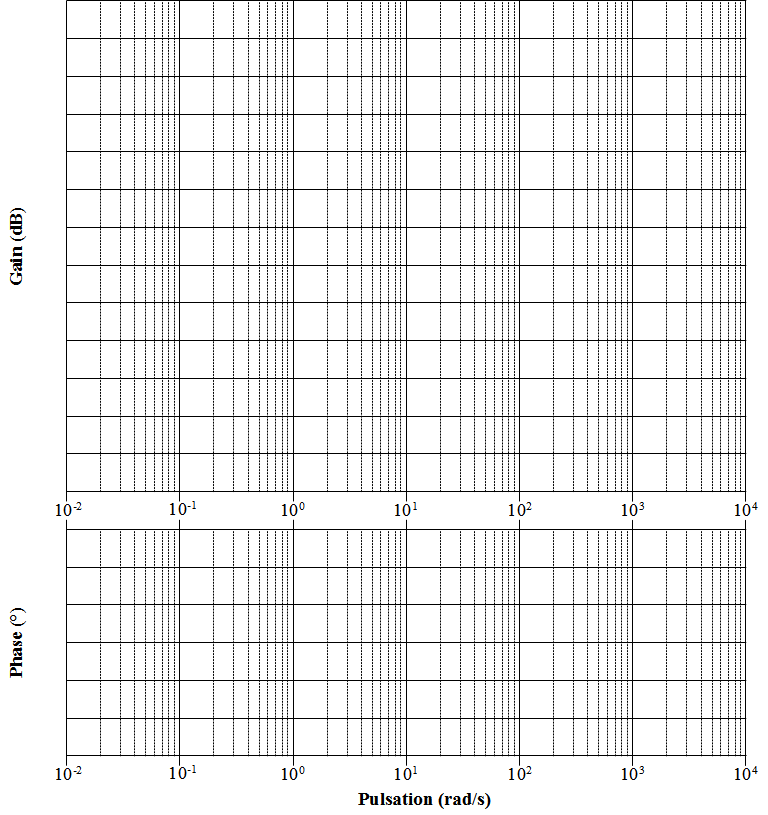
\includegraphics[width=.9\linewidth]{510_01}
\end{center}
\fi


\question{Tracer le diagramme de Bode de la fonction de transfert suivante : $F_2(p)=\dfrac{10}{\left(1+10p\right)\left(10+p\right)}$.}
\ifprof
\textbf{Tracer asymptotique}

$F_2(p)=\dfrac{1}{\left(1+10p\right)\left(1+\dfrac{p}{10}\right)}$

\begin{center}
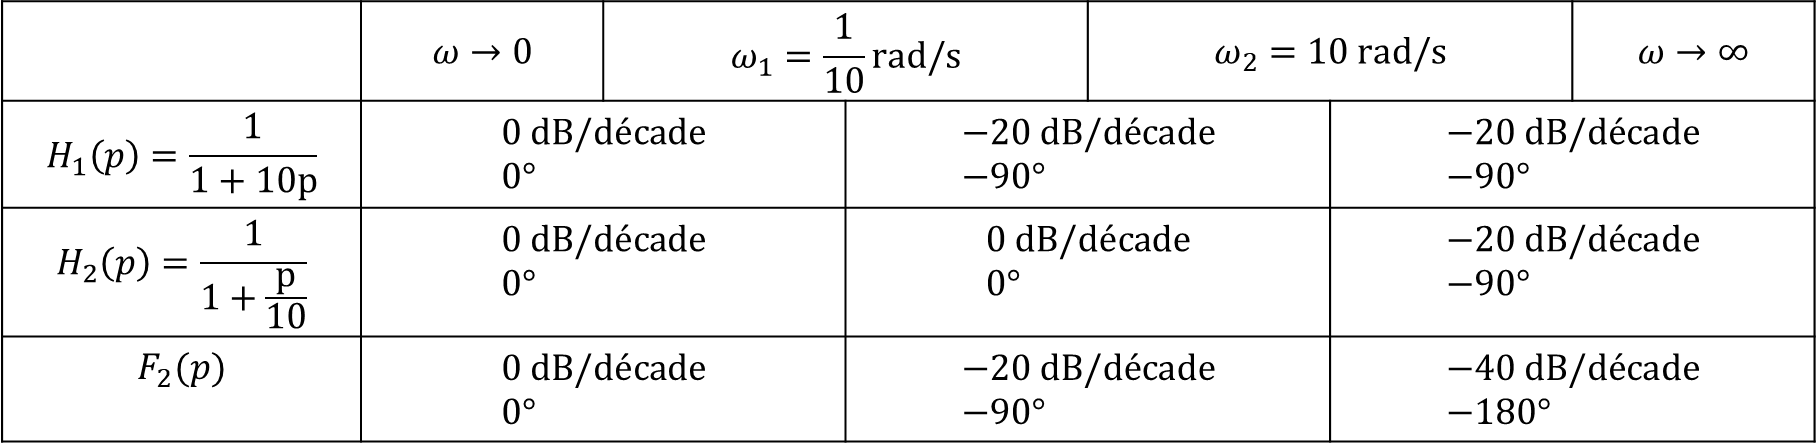
\includegraphics[width=.9\linewidth]{tab_02}
\end{center}


\textbf{Positionnement du diagramme de gain}
Lorsque que $\omega$ tend vers 0, le gain tend vers $20 \log 1 = \SI{0}{dB}$.

\begin{center}
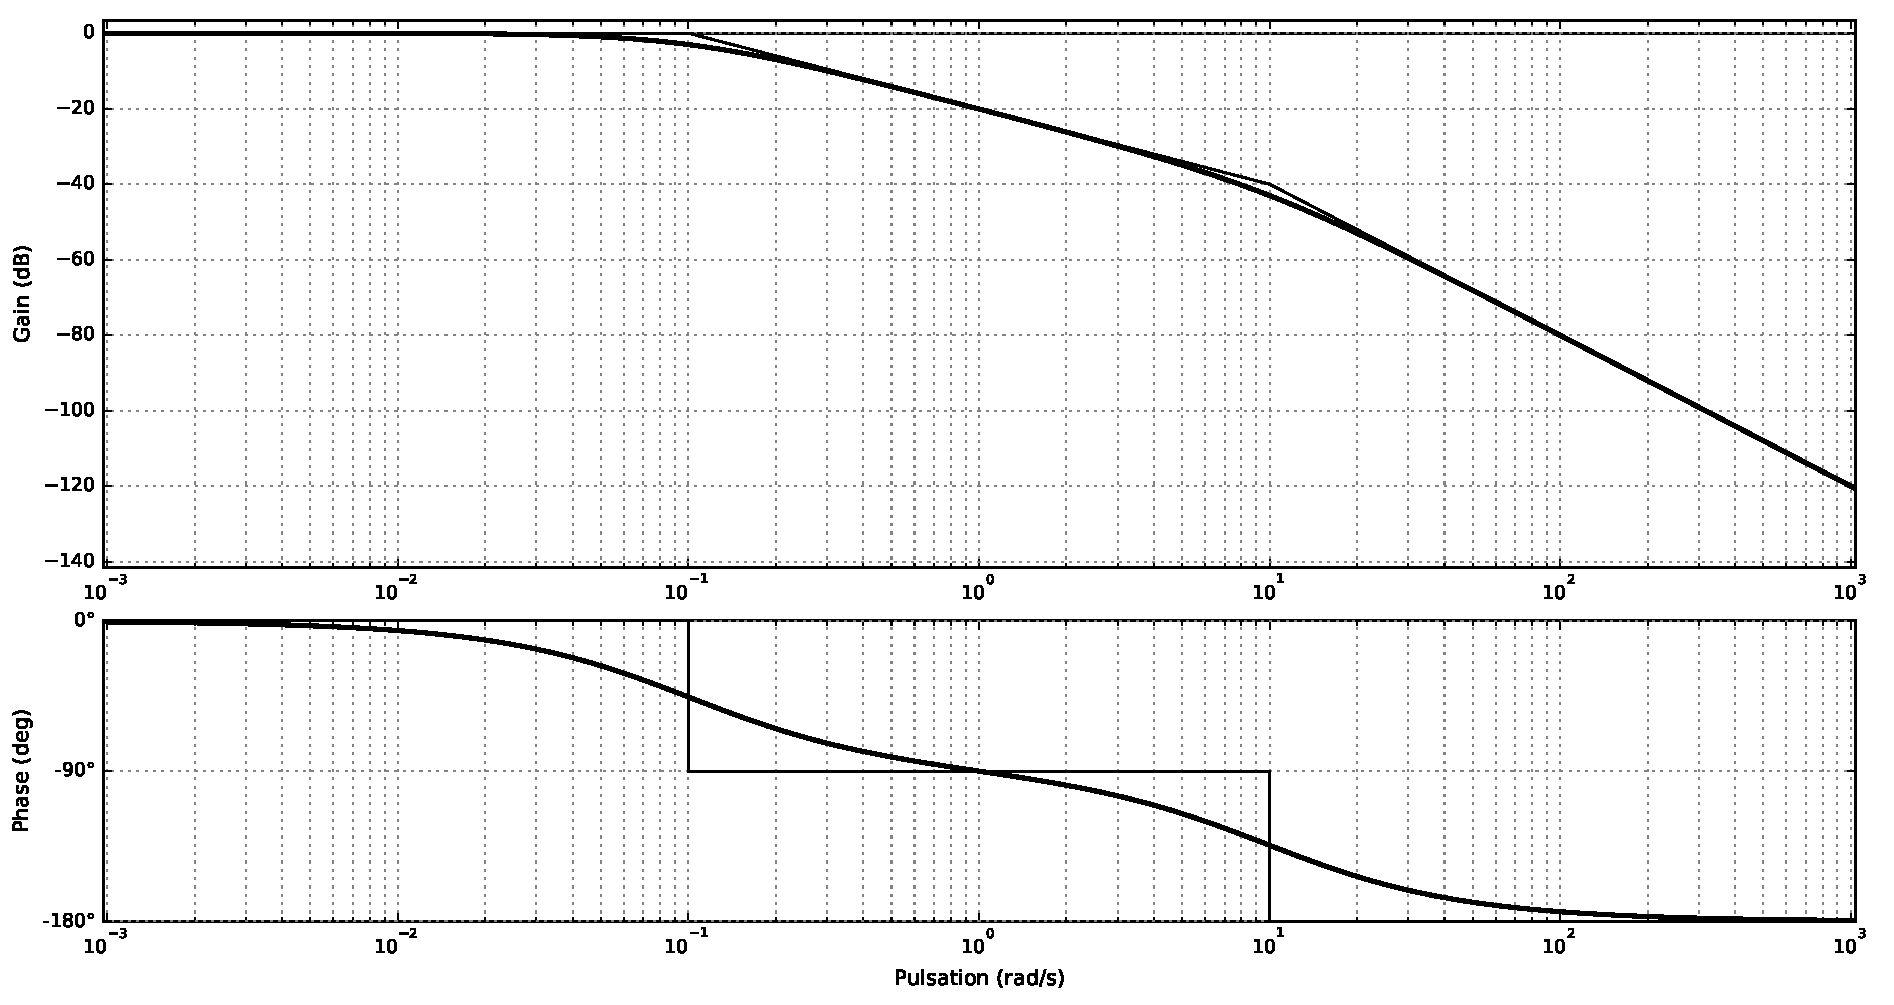
\includegraphics[width=.9\linewidth]{bode_02}
\end{center}

\else 
\begin{center}
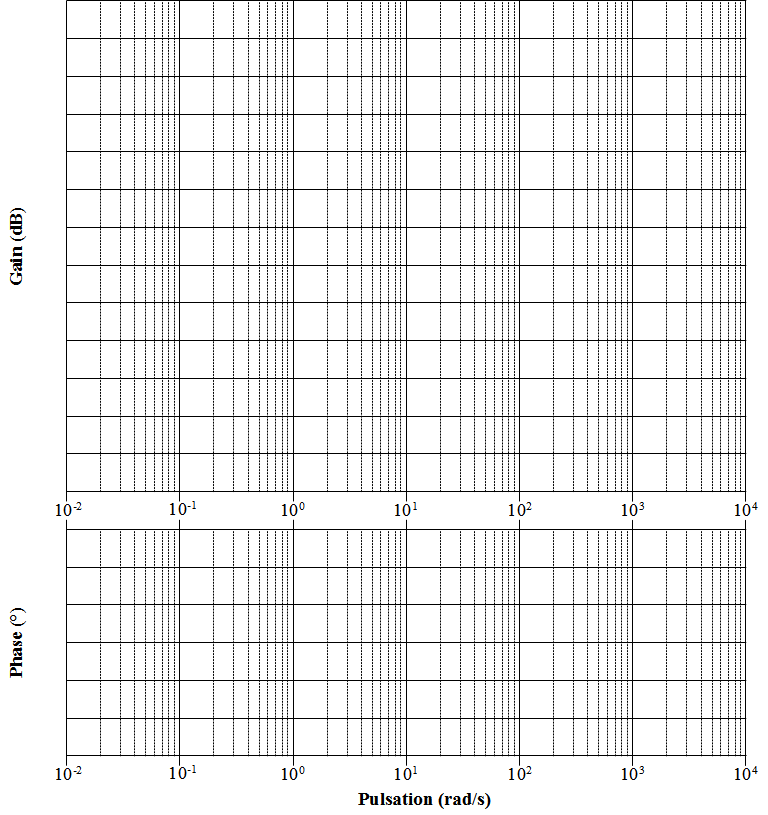
\includegraphics[width=.9\linewidth]{510_01}
\end{center}
\fi


\question{Tracer le diagramme de Bode de la fonction de transfert suivante : $F_3(p)=\dfrac{40}{p\left(1+300p\right)}$.}
\ifprof

\textbf{Tracer asymptotique}

\begin{center}
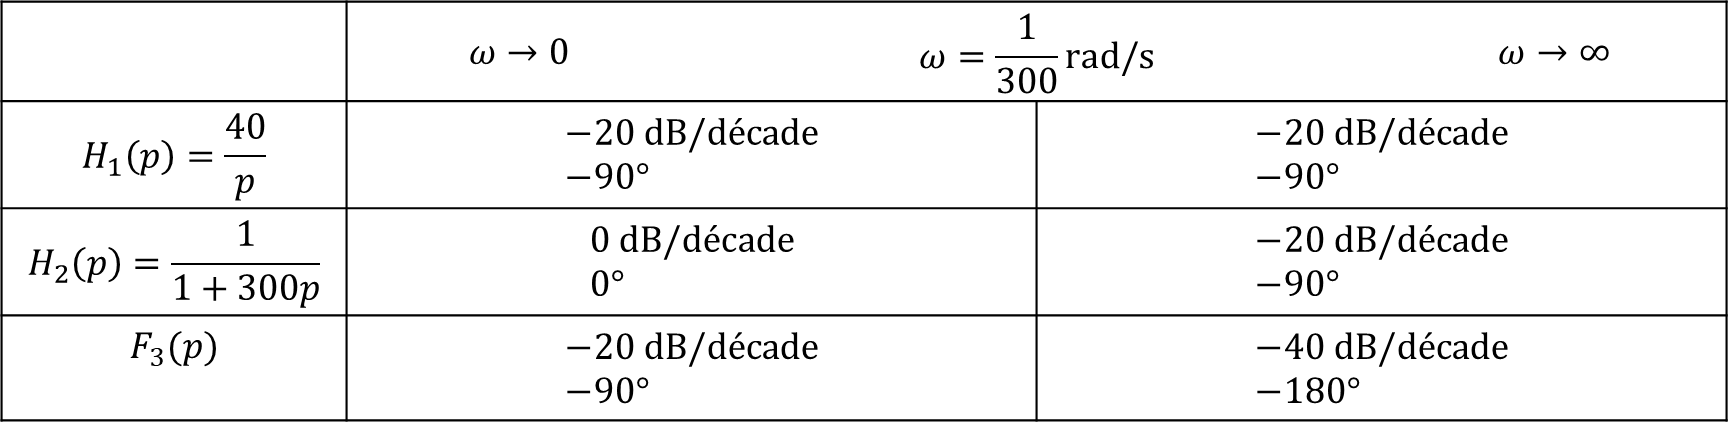
\includegraphics[width=.9\linewidth]{tab_03}
\end{center}


\textbf{Positionnement du diagramme de gain}
Lorsque que $\omega$ tend vers 0, $F_3(p)\simeq \dfrac{40}{p}$. Cette asymptote de pente \SI{-20}{dB/decade} passe par le point $(40,0)$. 

\begin{center}
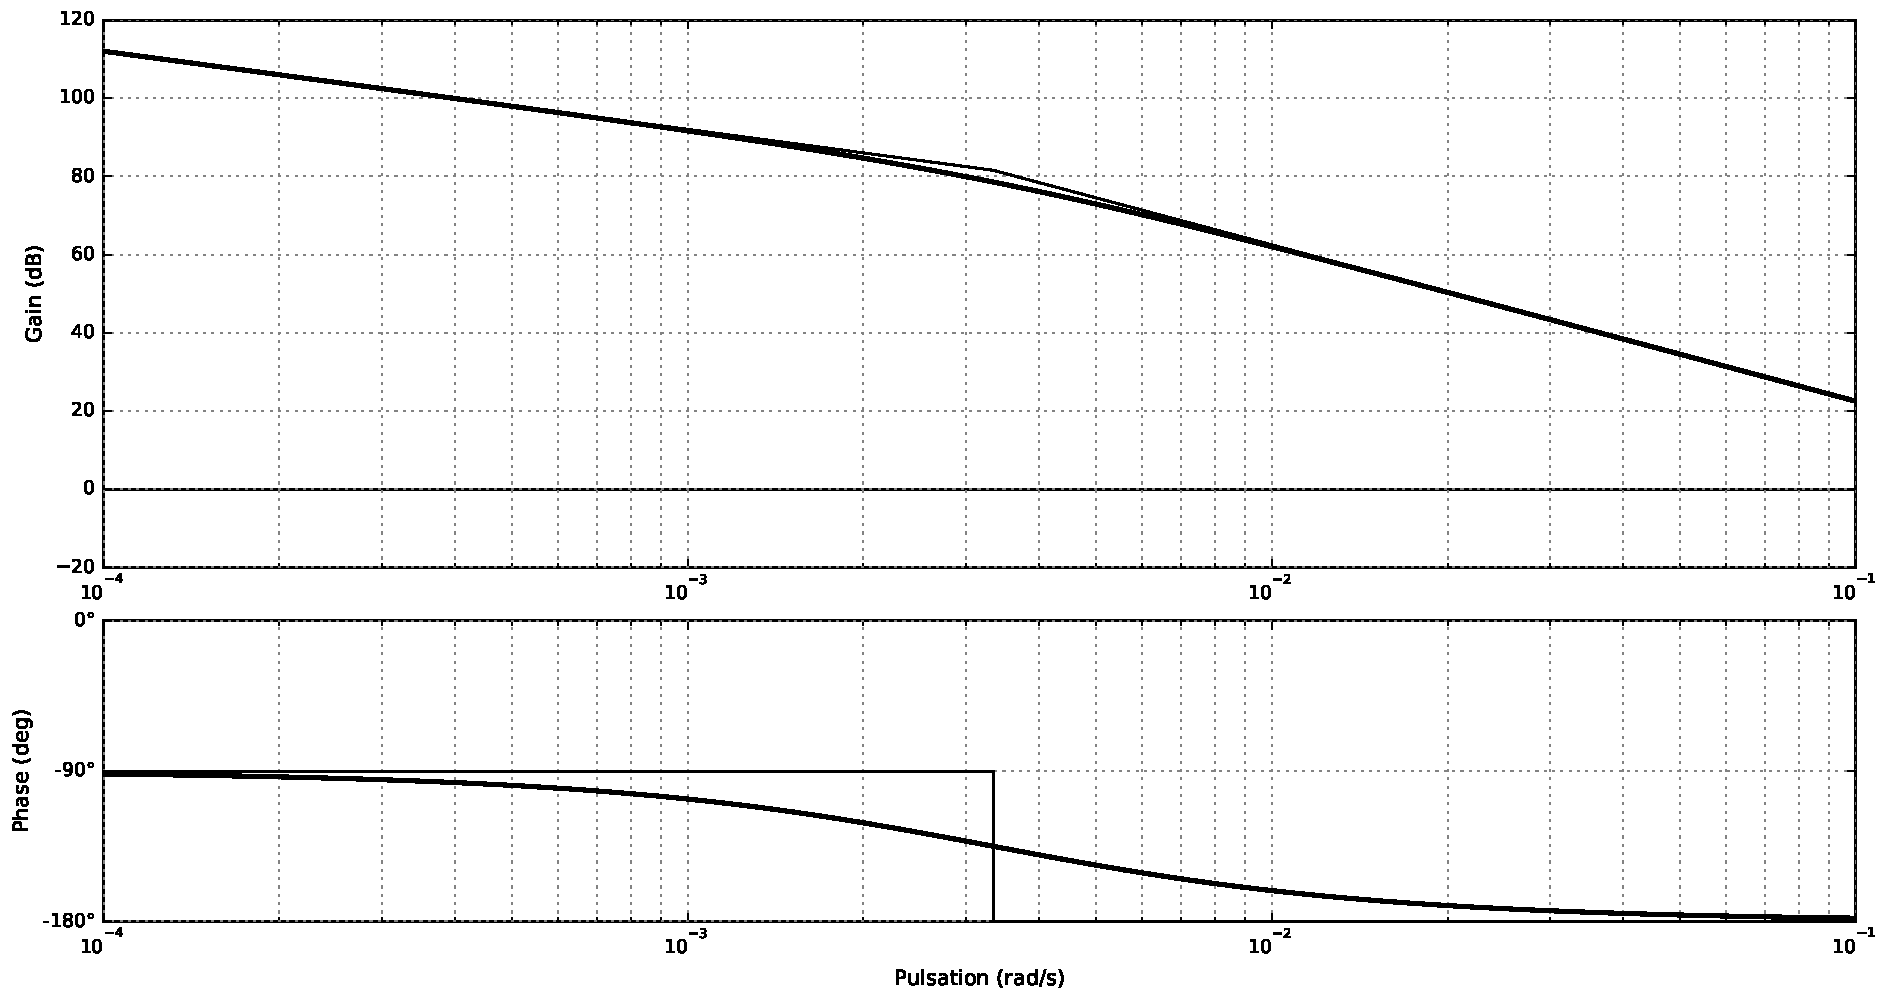
\includegraphics[width=.9\linewidth]{bode_03}
\end{center}

\else 
\begin{center}
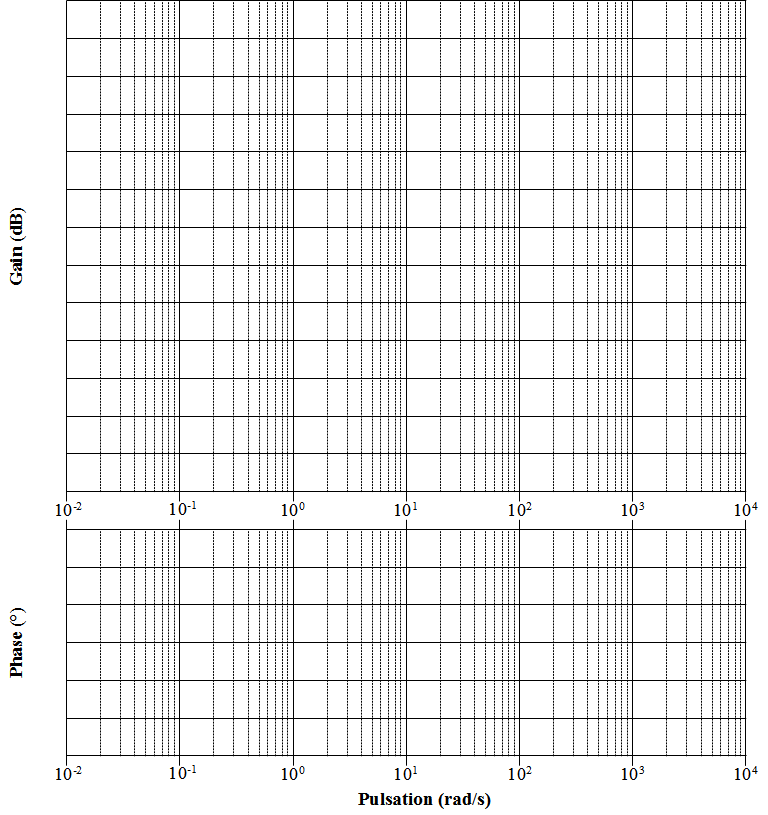
\includegraphics[width=.9\linewidth]{510_01}
\end{center}
\fi





%\question{Réaliser le schéma-blocs.}
%\ifprof
%\begin{figure}[H]
%\centering
%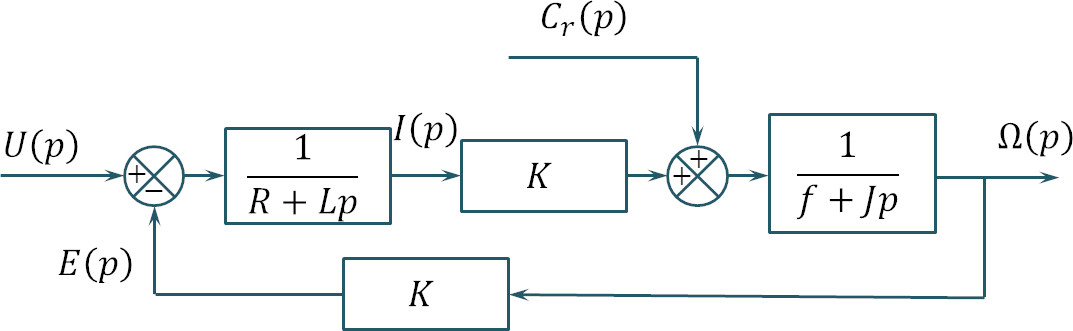
\includegraphics[width=\linewidth]{51_01_c}
%%\caption{Évolution du couple utile en fonction de la vitesse de rotation pour des
%%fréquences de commande de \SI{90}{Hz} à \SI{110}{Hz}. \label{fig_50_04}}
%\end{figure}
%\else
%\fi


 

\ifprof
\else
\begin{flushright}
\footnotesize{Corrigé  voir \ref{C2:02:510}.}
\end{flushright}%
\fi